\chapter{Introducción específica} % Main chapter title

\label{Chapter2}

En este capítulo se describen los elementos en los que se apoya el desarrollo del trabajo. En primer
lugar, se presentan las alteraciones acústicas que el sistema busca detectar. Luego, se mencionan
las herramientas y el entorno de cómputo utilizados, se describen las bases de datos públicas
empleadas para el entrenamiento y validación, y se presenta el modelo preentrenado utilizado como
punto de partida para la transferencia de aprendizaje.

%----------------------------------------------------------------------------------------

\section{Alteraciones acústicas buscadas}
\label{sec:alteraciones}

Como se mencionó en la sección \ref{sec:auscultacion}, cada patología modifica el sonido de
auscultación de una manera particular. En esta sección se describen las alteraciones que el sistema
debe reconocer tanto en tiempo como en frecuencia, ya que estas determinan qué información debe
conservar la representación de la señal.

\subsection{Alteraciones en los sonidos cardíacos}
\label{subsec:alteracionesCardiacas}

La alteración cardíaca considerada en este trabajo es el soplo. A diferencia de S1 y S2, que son
eventos breves, el soplo se prolonga durante parte de la sístole, de la diástole, o incluso durante
toda la fase. Por esa razón, se lo describe a partir de su ubicación dentro del ciclo cardíaco, su
forma, su tono, su calidad y su intensidad, que suele graduarse con la escala de Levine
\citep{oliveira2022circor}.

Los soplos son frecuentes en niños sanos y la mayoría no se debe a una patología. Sin embargo, un
soplo puede ser la única manifestación de una enfermedad cardíaca grave. Los soplos holosistólicos o
diastólicos, la intensidad de grado 3 o superior y la calidad áspera aumentan la probabilidad de que
el soplo sea patológico \citep{frank2011evaluation}. Las diferencias también se observan en el
espectro. En un estudio con 807 pacientes pediátricos, los soplos inocentes se concentraron
típicamente por debajo de los 200\,Hz, mientras que los patológicos abarcaron tanto frecuencias más
bajas como más altas \citep{noponen2007phono}.

En este trabajo, el modelo detecta la presencia de un soplo y no determina si es inocente o
patológico. Por lo tanto, una detección positiva no constituye un diagnóstico, sino una indicación
de que el paciente requiere una evaluación adicional por parte del profesional.

\subsection{Alteraciones en los sonidos pulmonares}
\label{subsec:alteracionesPulmonares}

Los sonidos adventicios pulmonares se dividen en discontinuos y continuos. Los crepitantes
pertenecen al primer grupo. Son eventos explosivos, de menos de 20\,ms de duración, cuya energía se
distribuye principalmente entre 60 y 1200\,Hz. Según la teoría, se producen cuando las pequeñas vías
aéreas colapsadas se abren de forma súbita durante la inspiración. Se clasifican en finos, que son
suaves, agudos y más numerosos en cada respiración, y gruesos, que son fuertes, graves y menos
numerosos. Los primeros se observan en enfermedades pulmonares intersticiales y los segundos, en la
bronquitis crónica \citep{sarkar2015auscultation}.

Las sibilancias pertenecen al grupo de los sonidos continuos. Son sonidos agudos, de carácter
musical, con una frecuencia dominante de 400\,Hz o más y una duración típicamente superior a
80-100\,ms. Se atribuyen a la oscilación de las paredes bronquiales provocada por el flujo de aire y
son características de la obstrucción generalizada de la vía aérea, como ocurre en el asma y en la
enfermedad pulmonar obstructiva crónica. Los roncus son sonidos continuos similares, pero más
graves, con una frecuencia dominante de alrededor de 200\,Hz o menos \citep{sarkar2015auscultation}.

Estas diferencias se reflejan en la representación tiempo-frecuencia, como se ilustra en la figura
\ref{fig:alteraciones}. El soplo ocupa el intervalo entre S1 y S2 con energía distribuida en un
rango amplio de frecuencias. Los crepitantes aparecen como trazos verticales breves y de banda
ancha. Las sibilancias, por su carácter tonal y sostenido, aparecen como trazos horizontales.

\begin{figure}[htbp]
	\centering
	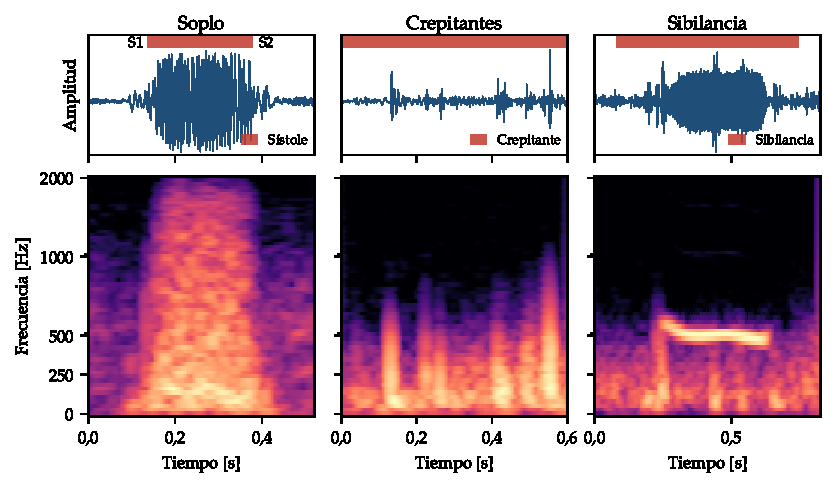
\includegraphics[width=\textwidth]{./Figures/alteraciones.pdf}
	\caption[Ejemplos de las alteraciones acústicas buscadas]{Forma de onda y espectrograma de
		un tramo de cada alteración buscada.}
	\label{fig:alteraciones}
\end{figure}

% \subsection{Clases consideradas}
% \label{subsec:clases}

% A partir de estas alteraciones, el modelo se diseñó para distinguir las siguientes seis clases:

% \begin{itemize}
% 	\item Sonido cardíaco normal.
% 	\item Sonido cardíaco con soplo.
% 	\item Sonido pulmonar normal.
% 	\item Sonido pulmonar con crepitantes.
% 	\item Sonido pulmonar con sibilancias.
% 	\item Sonido pulmonar con crepitantes y sibilancias.
% \end{itemize}

% Los crepitantes finos y gruesos se agruparon en una misma clase. Los roncus se incluyeron en la
% clase de sibilancias, ya que ambos son sonidos continuos. La última clase representa los casos en
% los que las dos alteraciones aparecen de forma conjunta. Además, esta agrupación permite unificar
% las etiquetas de las distintas bases de datos, que se describen en la sección
% \ref{sec:basesDatos}.

%----------------------------------------------------------------------------------------

\section{Herramientas y entorno de cómputo}
\label{sec:herramientas}

El trabajo se desarrolló en el lenguaje Python, que concentra la mayor parte de las bibliotecas de
aprendizaje automático y de procesamiento de audio. Los modelos se implementaron, entrenaron y
evaluaron con PyTorch \citep{paszke2019pytorch}. Para la lectura de las grabaciones, el remuestreo y
el cálculo de las representaciones tiempo-frecuencia se utilizó librosa \citep{mcfee2015librosa},
complementada con SciPy para el filtrado de las señales. Las métricas de evaluación se calcularon
con scikit-learn \citep{pedregosa2011scikit}, mientras que la manipulación de los datos y de los
metadatos de cada base se realizó con NumPy \citep{harris2020numpy} y pandas. Por último, las
figuras se generaron con Matplotlib.

% \begin{table}[htbp]
% 	\centering
% 	\caption[Herramientas de software utilizadas]{Herramientas de software utilizadas y su función
% 	en el trabajo.}
% 	\label{tab:herramientas}
% 	\small
% 	\begin{tabular}{l c l}
% 		\toprule
% 		\textbf{Herramienta} & \textbf{Versión} & \textbf{Uso} \\
% 		\midrule
% 		Python       & 3.12  & Lenguaje de programación \\
% 		PyTorch      & 2.13  & Definición, entrenamiento e inferencia de los modelos \\
% 		librosa      & 1.0   & Carga de audio, remuestreo y espectrogramas Mel \\
% 		SciPy        & 1.18  & Filtrado de señales \\
% 		scikit-learn & 1.9   & Métricas de evaluación \\
% 		NumPy        & 2.5   & Cálculo numérico \\
% 		pandas       & 3.0   & Manejo de datos tabulares y metadatos \\
% 		Matplotlib   & 3.11  & Generación de figuras \\
% 		\bottomrule
% 	\end{tabular}
% \end{table}

La mayor parte del trabajo se realizó en una computadora portátil con un procesador Intel Core
i7-1355U y 16\,GB de memoria RAM, sin una unidad de procesamiento gráfico (GPU, \textit{Graphics
Processing Unit}) dedicada. En ella se ejecutaron el preprocesamiento de los datos, el entrenamiento
de los modelos y la evaluación de los mismos. Para el ajuste fino del modelo preentrenado, cuyo
costo de cómputo resultaba inviable sin aceleración por hardware, se utilizó Google Colab, una
plataforma en la nube que ofrece notebooks de Python con acceso a GPU. En particular, se empleó una
GPU NVIDIA Tesla T4.

%----------------------------------------------------------------------------------------

\section{Bases de datos}
\label{sec:basesDatos}

Se utilizaron cuatro bases de datos públicas, cuyas características se resumen en la tabla
\ref{tab:basesDatos}. Dos de ellas, CirCor DigiScope y SPRSound, se emplearon para entrenar y
evaluar los modelos. Ambas están compuestas por grabaciones de pacientes pediátricos, una para los
sonidos cardíacos y otra para los pulmonares. Las otras dos, ICBHI 2017 y HLS-CMDS, se reservaron
para evaluar los modelos con datos provenientes de otras poblaciones y de otros equipos de
grabación. No se utilizaron datos propios.

\begin{table}[!htb]
	\centering
	\caption[Características de las bases de datos utilizadas]{Características de las bases de
		datos utilizadas.}
	\label{tab:basesDatos}
	\small
	\begin{tabular}{>{\raggedright\arraybackslash}p{1.9cm} >{\raggedright\arraybackslash}p{2.4cm} >{\raggedright\arraybackslash}p{2.4cm} >{\raggedright\arraybackslash}p{2.4cm} >{\raggedright\arraybackslash}p{2.3cm}}
		\toprule
		 & \textbf{CirCor DigiScope} & \textbf{SPRSound} & \textbf{ICBHI 2017} & \textbf{HLS-CMDS} \\
		\midrule
		Uso & Entrenamiento & Entrenamiento & Validación externa & Validación externa \\
		\addlinespace
		Sonido & Cardíaco & Pulmonar & Pulmonar & Cardíaco, pulmonar y mezclas \\
		\addlinespace
		Origen & Paraíba, Brasil & Shanghái, China & Portugal y Grecia & Maniquí clínico \\
		\addlinespace
		Población & Pediátrica (neonatos a adolescentes) & Pediátrica (0 a 16,8 años) & Todas las edades (0,25 a 93 años) & No aplica \\
		\addlinespace
		Pacientes & 942 & 952 & 126 & No aplica \\
		\addlinespace
		Grabaciones & 3163 & 6567 & 920 & 535 \\
		\addlinespace
		Duración total & 20,1\,h & 20,8\,h & 5,5\,h & 2,2\,h \\
		\addlinespace
		Frecuencia de muestreo & 4\,kHz & 8\,kHz & 4, 10 y 44,1\,kHz & 4\,kHz \\
		\addlinespace
		Anotación & Soplo por paciente; segmentación del ciclo cardíaco & Etiqueta por grabación; eventos con inicio y fin & Crepitantes y sibilancias por ciclo respiratorio & Tipo de sonido por grabación \\
		\addlinespace
		Licencia & ODC-By 1.0 & CC BY 4.0 & Libre acceso para investigación & MIT \\
		\bottomrule
	\end{tabular}
\end{table}

\subsection{CirCor DigiScope}
\label{subsec:circor}

La base CirCor DigiScope reúne grabaciones fonocardiográficas obtenidas durante dos campañas de
tamizaje realizadas en el estado de Paraíba, Brasil, en 2014 y 2015, con un estetoscopio electrónico
Littmann 3200 \citep{oliveira2022circor}. Cada paciente fue auscultado principalmente en cuatro
focos, que corresponden a las válvulas aórtica, pulmonar, tricuspídea y mitral, por lo que tiene
varias grabaciones asociadas. En este trabajo se utilizó la porción pública de la base, que
corresponde al conjunto de entrenamiento del George B. Moody PhysioNet Challenge 2022
\citep{reyna2023heart}.

Las anotaciones se realizan por paciente. Para cada uno se indica si presenta un soplo, si no lo
presenta o si la calidad de las grabaciones no permitió determinarlo. En los casos con soplo se
agregan los focos en los que se escucha y sus características, descritas en la sección
\ref{subsec:alteracionesCardiacas}. Además, cada grabación incluye una segmentación del ciclo
cardíaco, que marca el inicio y el fin de S1, de la sístole, de S2 y de la diástole.

\subsection{SPRSound}
\label{subsec:sprsound}

SPRSound es una base de sonidos respiratorios pediátricos registrados con un estetoscopio digital
Yunting modelo II en el Shanghai Children's Medical Center, un hospital pediátrico de China
\citep{zhang2022sprsound}. Su primera versión, publicada en 2022, contenía 2683 grabaciones de 292
pacientes. La base se amplió luego con las entregas de las ediciones 2023, 2024 y 2025 del desafío
de sonidos respiratorios de la conferencia IEEE BioCAS. En este trabajo se utilizaron todas las
entregas disponibles.

Cada grabación tiene dos niveles de anotación. A nivel de grabación se la clasifica como normal, con
sonidos adventicios continuos, con sonidos adventicios discontinuos, con ambos tipos o de mala
calidad. A nivel de evento se marcan el inicio y el fin de cada segmento y su tipo: normal,
crepitante fino, crepitante grueso, sibilancia, roncus, estridor o sibilancia con crepitante. Las
anotaciones fueron realizadas por un equipo de once médicos pediatras \citep{zhang2022sprsound}.

\subsection{ICBHI 2017}
\label{subsec:icbhi}

La base del desafío ICBHI 2017 contiene grabaciones de sonidos respiratorios de pacientes de todas
las edades, registradas en Portugal y en Grecia con cuatro equipos distintos, entre estetoscopios
electrónicos y micrófonos \citep{rocha2019open}. Cada grabación se divide en ciclos respiratorios, y
para cada ciclo se indica la presencia de crepitantes y de sibilancias. La base incluye además el
diagnóstico de cada paciente. Predomina la enfermedad pulmonar obstructiva crónica, con 64 de los
126 pacientes, seguida por 26 pacientes sanos y 14 con infección del tracto respiratorio superior.
Como se mencionó en la sección \ref{sec:estadoArte}, es la referencia más utilizada para comparar
algoritmos de clasificación de sonidos respiratorios.

\subsection{HLS-CMDS}
\label{subsec:hls}

HLS-CMDS es una base grabada sobre un maniquí clínico que reproduce sonidos cardíacos y pulmonares,
normales y patológicos, registrados con un estetoscopio digital en distintos puntos del tórax
\citep{torabi2025hlscmds}. Contiene 50 grabaciones de sonidos cardíacos, 50 de sonidos pulmonares y
145 mezclas de ambos. Para cada mezcla se incluyen también sus dos componentes grabados por
separado. Al no provenir de pacientes, sus sonidos son más controlados que los de una auscultación
real, pero permiten evaluar el comportamiento de los modelos ante un equipo de grabación y unas
condiciones que no forman parte del entrenamiento.

%----------------------------------------------------------------------------------------

\section{Modelo preentrenado}
\label{sec:preentrenado}

La transferencia de aprendizaje consiste en reutilizar una red entrenada sobre un conjunto de datos
grande para resolver una tarea distinta, en la que los datos disponibles son menos. Las primeras
capas de una red convolucional aprenden patrones generales de la señal, como bordes, texturas o
componentes de frecuencia, que pueden aprovecharse en otros problemas. Existen dos formas habituales
de aplicarla: utilizar la red preentrenada como extractor de características, con sus parámetros
congelados, y entrenar solo un clasificador sobre ella, o bien utilizarla como punto de partida y
ajustar una parte de sus parámetros con los datos de la nueva tarea, lo que se conoce como ajuste
fino o \textit{fine-tuning} \citep{kong2020panns}.

En este trabajo se utilizó como modelo preentrenado la red CNN6 de la familia PANNs
(\textit{Pretrained Audio Neural Networks}) \citep{kong2020panns}. Las PANNs son redes entrenadas
para el etiquetado de eventos sonoros sobre AudioSet, un conjunto de más de dos millones de
fragmentos de audio de 10\,s extraídos de videos de YouTube y etiquetados según una ontología de 527
clases, que incluye voz, música, sonidos de animales, sonidos ambientales y sonidos del cuerpo
humano, entre otras \citep{gemmeke2017audioset}. Sus autores entrenaron las redes con unos 1,9
millones de esos fragmentos y publicaron los pesos resultantes, lo que permite utilizarlas como
punto de partida en otras tareas de audio. La tabla \ref{tab:cnn6} resume las características de la
CNN6, la red convolucional más pequeña de la familia, que se eligió porque su tamaño resulta
compatible con los recursos de cómputo descritos en la sección \ref{sec:herramientas}.

\begin{table}[htbp]
	\centering
	\caption[Características del modelo preentrenado CNN6]{Características del modelo
		preentrenado CNN6 de la familia PANNs.}
	\label{tab:cnn6}
	\small
	\begin{tabular}{>{\raggedright\arraybackslash}p{4.2cm} >{\raggedright\arraybackslash}p{8.2cm}}
		\toprule
		\textbf{Característica} & \textbf{Valor} \\
		\midrule
		Arquitectura & 4 capas convolucionales de $5 \times 5$ con 64, 128, 256 y 512 filtros, cada una con normalización por lotes, ReLU y promedio de $2 \times 2$ \\
		\addlinespace
		Agregación y salida & Suma del promedio y el máximo global, capa de 512 unidades y salida de 527 clases \\
		\addlinespace
		Parámetros & 4,8 millones \\
		\addlinespace
		Datos de preentrenamiento & AudioSet: 1,9 millones de fragmentos de 10\,s, 527 clases \\
		\addlinespace
		Entrada & Espectrograma log-Mel de 64 bandas entre 50\,Hz y 14\,kHz, calculado a 32\,kHz con ventanas de 1024 muestras y saltos de 320 \\
		\addlinespace
		Aumentación en el preentrenamiento & \textit{Mixup} y SpecAugment \\
		\addlinespace
		Desempeño en AudioSet & Precisión media promedio (mAP) de 0,343 \\
		\bottomrule
	\end{tabular}
\end{table}

% Los sonidos de AudioSet difieren de los de auscultación. Se trata de audio de uso general,
% muestreado a 32\,kHz, mientras que las bases de entrenamiento de este trabajo están muestreadas a
% 4 y 8\,kHz (tabla \ref{tab:basesDatos}) y las alteraciones buscadas ocupan principalmente la parte
% baja del espectro, como se describió en la sección \ref{sec:alteraciones}. Por lo tanto, para
% utilizar la CNN6 fue necesario adaptar la representación de entrada y la capa de salida a la tarea
% de este trabajo. El modo en que se realizó esa adaptación y el ajuste fino se describen en el
% capítulo \ref{Chapter3}.

% %----------------------------------------------------------------------------------------
% %	SECTION 1
% %----------------------------------------------------------------------------------------
% Todos los capítulos deben comenzar con un breve párrafo introductorio que indique cuál es el
% contenido que se encontrará al leerlo.  La redacción sobre el contenido de la memoria debe hacerse
% en presente y todo lo referido al proyecto en pasado, siempre de modo impersonal.

% \section{Estilo y convenciones}
% \label{sec:ejemplo}

% \subsection{Uso de mayúscula inicial para los título de secciones}

% Si en el texto se hace alusión a diferentes partes del trabajo referirse a ellas como capítulo,
% sección o subsección según corresponda. Por ejemplo: ``En el capítulo \ref{Chapter1} se explica
% tal cosa'', o ``En la sección \ref{sec:ejemplo} se presenta lo que sea'', o ``En la subsección
% \ref{subsec:ejemplo} se discute otra cosa''.

% Cuando se quiere poner una lista tabulada, se hace así:

% \begin{itemize}
% 	\item Este es el primer elemento de la lista.
% 	\item Este es el segundo elemento de la lista.
% \end{itemize}

% Notar el uso de las mayúsculas y el punto al final de cada elemento.

% Si se desea poner una lista numerada el formato es este:

% \begin{enumerate}
% 	\item Este es el primer elemento de la lista.
% 	\item Este es el segundo elemento de la lista.
% \end{enumerate}

% Notar el uso de las mayúsculas y el punto al final de cada elemento.

% \subsection{Este es el título de una subsección}
% \label{subsec:ejemplo}

% Se recomienda no utilizar \textbf{texto en negritas} en ningún párrafo, ni tampoco texto
% \underline{subrayado}. En cambio sí se debe utilizar \textit{texto en itálicas} para palabras en
% un idioma extranjero, al menos la primera vez que aparecen en el texto. En el caso de palabras que
% estamos inventando se deben utilizar ``comillas'', así como también para citas textuales. Por
% ejemplo, un \textit{digital filter} es una especie de ``selector'' que permite separar ciertos
% componentes armónicos en particular.

% La escritura debe ser impersonal. Por ejemplo, no utilizar ``el diseño del firmware lo hice de
% acuerdo con tal principio'', sino ``el firmware fue diseñado utilizando tal principio''.

% El trabajo es algo que al momento de escribir la memoria se supone que ya está concluido, entonces
% todo lo que se refiera a hacer el trabajo se narra en tiempo pasado, porque es algo que ya
% ocurrió. Por ejemplo, "se diseñó el firmware empleando la técnica de test driven development".

% En cambio, la memoria es algo que está vivo cada vez que el lector la lee. Por eso transcurre
% siempre en tiempo presente, como por ejemplo:

% ``En el presente capítulo se da una visión global sobre las distintas pruebas realizadas y los
% resultados obtenidos. Se explica el modo en que fueron llevados a cabo los test unitarios y las
% pruebas del sistema''.

% Se recomienda no utilizar una sección de glosario sino colocar la descripción de las abreviaturas
% como parte del mismo cuerpo del texto. Por ejemplo, RTOS (\textit{Real Time Operating System},
% Sistema Operativo de Tiempo Real) o en caso de considerarlo apropiado mediante notas a pie de
% página.

% Si se desea indicar alguna página web utilizar el siguiente formato de referencias bibliográficas,
% dónde las referencias se detallan en la sección de bibliografía de la memoria, utilizado el
% formato establecido por IEEE en \citep{IEEE:citation}. Por ejemplo, ``el presente trabajo se basa
% en la plataforma EDU-CIAA-NXP \citep{CIAA}, la cual...''.

% \subsection{Figuras} 

% Al insertar figuras en la memoria se deben considerar determinadas pautas. Para empezar, usar
% siempre tipografía claramente legible. Luego, tener claro que \textbf{es incorrecto} escribir por
% ejemplo esto: ``El diseño elegido es un cuadrado, como se ve en la siguiente figura:''

% \begin{figure}[h]
% \centering
% 
\includegraphics[scale=.45]{./Figures/cuadradoAzul.png}
% \end{figure}

% La forma correcta de utilizar una figura es con referencias cruzadas, por ejemplo: ``Se eligió
% utilizar un cuadrado azul para el logo, como puede observarse en la figura
% \ref{fig:cuadradoAzul}''.

% \begin{figure}[ht]
% 	\centering
% 	
\includegraphics[scale=.45]{./Figures/cuadradoAzul.png}
% 	\caption{Ilustración del cuadrado azul que se eligió para el diseño del logo.}
% 	\label{fig:cuadradoAzul}
% \end{figure}

% El texto de las figuras debe estar siempre en español, excepto que se decida reproducir una figura
% original tomada de alguna referencia. En ese caso la referencia de la cual se tomó la figura debe
% ser indicada en el epígrafe de la figura e incluida como una nota al pie, como se ilustra en la
% figura \ref{fig:palabraIngles}.

% \begin{figure}[htpb]
% 	\centering
% 	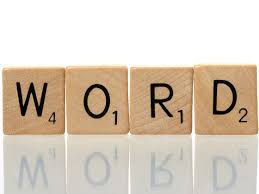
\includegraphics[scale=.3]{./Figures/word.jpeg}
% 	\caption{Imagen tomada de la página oficial del procesador\protect\footnotemark.}
% 	\label{fig:palabraIngles}
% \end{figure}

% \footnotetext{Imagen tomada de \url{https://goo.gl/images/i7C70w}}

% La figura y el epígrafe deben conformar una unidad cuyo significado principal pueda ser
% comprendido por el lector sin necesidad de leer el cuerpo central de la memoria. Para eso es
% necesario que el epígrafe sea todo lo detallado que corresponda y si en la figura se utilizan
% abreviaturas entonces aclarar su significado en el epígrafe o en la misma figura.



% \begin{figure}[ht]
% 	\centering
% 	
\includegraphics[scale=.37]{./Figures/questionMark.png}
% 	\caption{¿Por qué de pronto aparece esta figura?}
% 	\label{fig:questionMark}
% \end{figure}

% Nunca colocar una figura en el documento antes de hacer la primera referencia a ella, como se
% ilustra con la figura \ref{fig:questionMark}, porque sino el lector no comprenderá por qué de
% pronto aparece la figura en el documento, lo que distraerá su atención.

% Otra posibilidad es utilizar el entorno \textit{subfigure} para incluir más de una figura, como se
% puede ver en la figura \ref{fig:three graphs}. Notar que se pueden referenciar también las figuras
% internas individualmente de esta manera: \ref{fig:1de3}, \ref{fig:2de3} y \ref{fig:3de3}.
 
% \begin{figure}[!htpb]
%      \centering
%      \begin{subfigure}[b]{0.3\textwidth}
%          \centering
%          
\includegraphics[width=.65\textwidth]{./Figures/questionMark}
%          \caption{Un caption.}
%          \label{fig:1de3}
%      \end{subfigure}
%      \hfill
%      \begin{subfigure}[b]{0.3\textwidth}
%          \centering
%          
\includegraphics[width=.65\textwidth]{./Figures/questionMark}
%          \caption{Otro.}
%          \label{fig:2de3}
%      \end{subfigure}
%      \hfill
%      \begin{subfigure}[b]{0.3\textwidth}
%          \centering
%          
\includegraphics[width=.65\textwidth]{./Figures/questionMark}
%          \caption{Y otro más.}
%          \label{fig:3de3}
%      \end{subfigure}
%         \caption{Tres gráficos simples.}
%         \label{fig:three graphs}
% \end{figure}

% El código para generar las imágenes se encuentra disponible para su reutilización en el archivo
% \file{Chapter2.tex}.

% \subsection{Tablas}

% Para las tablas utilizar el mismo formato que para las figuras, sólo que el epígrafe se debe
% colocar arriba de la tabla, como se ilustra en la tabla \ref{tab:peces}. Observar que sólo algunas
% filas van con líneas visibles y notar el uso de las negritas para los encabezados.  La referencia
% se logra utilizando el comando \verb|\ref{<label>}| donde label debe estar definida dentro del
% entorno de la tabla.

% \begin{verbatim}
% \begin{table}[h]
% 	\centering
% 	\caption[caption corto]{caption largo más descriptivo}
% 	\begin{tabular}{l c c}    
% 		\toprule
% 		\textbf{Especie}     & \textbf{Tamaño} & \textbf{Valor}\\
% 		\midrule
% 		Amphiprion Ocellaris & 10 cm           & \$ 6.000 \\		
% 		Hepatus Blue Tang    & 15 cm           & \$ 7.000 \\
% 		Zebrasoma Xanthurus  & 12 cm           & \$ 6.800 \\
% 		\bottomrule
% 		\hline
% 	\end{tabular}
% 	\label{tab:peces}
% \end{table}
% \end{verbatim}


% \begin{table}[h]
% 	\centering
% 	\caption[caption corto]{caption largo más descriptivo.}
% 	\begin{tabular}{l c c}    
% 		\toprule
% 		\textbf{Especie} 	 & \textbf{Tamaño} 		& \textbf{Valor}  \\
% 		\midrule
% 		Amphiprion Ocellaris & 10 cm 				& \$ 6.000 \\		
% 		Hepatus Blue Tang	 & 15 cm				& \$ 7.000 \\
% 		Zebrasoma Xanthurus	 & 12 cm				& \$ 6.800 \\
% 		\bottomrule
% 		\hline
% 	\end{tabular}
% 	\label{tab:peces}
% \end{table}

% En cada capítulo se debe reiniciar el número de conteo de las figuras y las tablas, por ejemplo,
% figura 2.1 o tabla 2.1, pero no se debe reiniciar el conteo en cada sección. Por suerte la
% plantilla se encarga de esto por nosotros.

% \subsection{Ecuaciones}
% \label{sec:Ecuaciones}

% Al insertar ecuaciones en la memoria dentro de un entorno \textit{equation}, éstas se numeran en
% forma automática  y se pueden referir al igual que como se hace con las figuras y tablas, por
% ejemplo ver la ecuación \ref{eq:metric}.

% \begin{equation}
% 	\label{eq:metric}
% 	ds^2 = c^2 dt^2 \left( \frac{d\sigma^2}{1-k\sigma^2} + \sigma^2\left[ d\theta^2 + \sin^2\theta
% 	d\phi^2 \right] \right)
% \end{equation}
                                                        
% Para generar la ecuación \ref{eq:metric} se utilizó el siguiente código:

% \begin{verbatim}
% \begin{equation}
% 	\label{eq:metric}
% 	ds^2 = c^2 dt^2 \left( \frac{d\sigma^2}{1-k\sigma^2} + 
% 	\sigma^2\left[ d\theta^2 + 
% 	\sin^2\theta d\phi^2 \right] \right)
% \end{equation}
% \end{verbatim}
